\section{Introduction}

The process of conversion of Alternating current into Direct current is known as rectification. For this, Diodes --- which only allow unidirectional flow of current --- are used. In this experiment, we are making a half-wave rectifier.

\section{Theory}
In a a Half-wave rectifier, during the positive half-cycle of the AC input, the diode is forward biased and current flows through the load and a voltage is developed across it. During the negative half-cycle, it is reverse biased and does not conduct. Therefore, no current flows in the load resistor as no voltage appears across it.

Thus the DC voltage across the load is sinusoidal for the first half cycle only and a pure A.C. input signal is converted into a unidirectional pulsating output signal.

We can represent the input AC voltage by 

\begin{equation*}
    V(t) = V_\text{max}\sin(\omega t)   
\end{equation*}

Since the diode conducts only in one half-cycle (0-$\pi$), the DC component in the output will be the time average of $V(t)$ from $0$ to $T/2$, $\left<V(t)\right>$ which comes out to be $V_\text{max}/\pi$, where $V_\text{max}$ is the peak value of the voltage.

\begin{equation}
    V_{\text{dc}} = \left<V(t)\right> = \frac{V_{\text{max}}}{\pi} = 0.318V_\text{max}
\end{equation}

The RMS of voltage would be,

\begin{equation}
    V_{\text{rms}} = \left<V^2(t)\right> = \frac{V_{\text{max}}}{2}
\end{equation}

\begin{figure}[H]
    \centering
    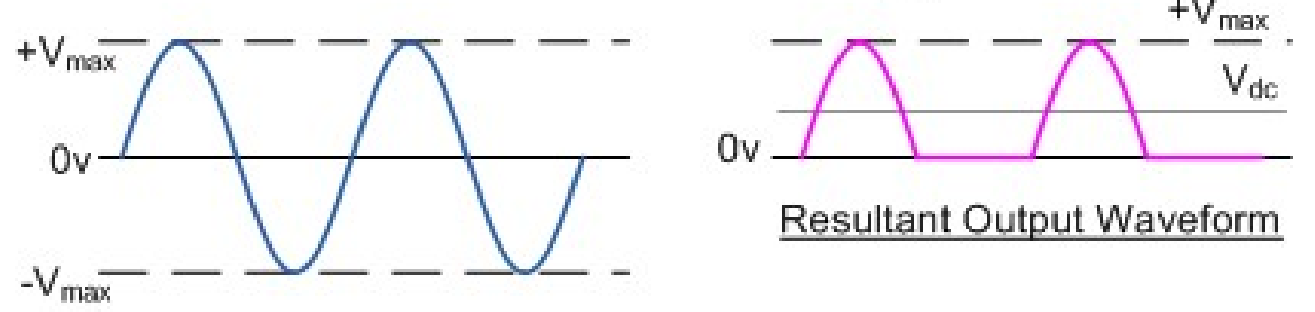
\includegraphics[width=1\columnwidth]{images/f1.png}
    \caption{Half-wave rectifier input and output waveforms}
\end{figure}

\subsection{Ripple Factor}
As the voltage across the load resistor is only present during the positive half of the cycle, the average DC voltage measured is very low.This variation on the rectified waveform is called \textit{Ripple} and is an undesirable feature. The ripple factor is a measure of purity of the d.c. output of a rectifier and is defined as:
\newcommand{\at}[2][]{#1|_{#2}}
\begin{equation}
    r = \frac{V_\text{ac}}{V_\text{dc}}
\end{equation}

Where $V_\text{ac}$ and $V_\text{ac}$ are the AC and DC components of the output wavform respectively. Since $V^2_\text{rms} = V^2_\text{ac} + V^2_\text{dc}$,

\begin{align*}
    r &= \sqrt{\frac{V^2_\text{rms} - V^2_\text{dc}}{V^2_\text{dc}}}\\
    &= \sqrt{\frac{V^2_\text{rms}}{V^2_\text{dc}}-1} = \sqrt{\frac{0.5}{0.318}-1}\\ &= 1.21
\end{align*}

\subsection{Rectification Efficiency}
Rectification efficiency ($\eta$), is a measure of the percentage of total AC power input converted to useful DC power output. 

\begin{align*}
    \eta &= \frac{V_\text{dc}I_\text{dc}}{V_\text{ac}I_\text{ac}}
    = \frac{I^2_\text{dc}R}{I^2_\text{ac}/(r_d+R)}\\
    &=\frac{(0.318V_\text{max})^2}{(0.5V_\text{max})^2\left(1+\frac{r_d}{R}\right)} = \frac{0.405}{\left(1+\frac{r_d}{R}\right)}
\end{align*}

where $r_d$ is the forward resistance of the diode. Under ideal conditions ($r_d \approx 0$), the rectification efficiency for a half-wave rectifier is 40.5\%.

\subsection{Filters}
The output of a rectifier gives a pulsating DC signal because of presence of some AC components whose frequency is equal to that of the AC supply frequency. To remove any voltage variations or ripples, and smoothen the output, Filter circuits are used. 
Various filter circuits are available such as shunt capacitor, series inductor, choke input LC filter and $\pi$-filter etc. Here we use a simple shunt capacitor filter circuit. Since a capacitor is open to DC and offers low impedance path to AC current, putting a capacitor across the output will make the DC component to pass through the load resulting in smaller ripple voltage. 

\subsubsection{Working Principle}

\begin{figure}[H]
    \centering
    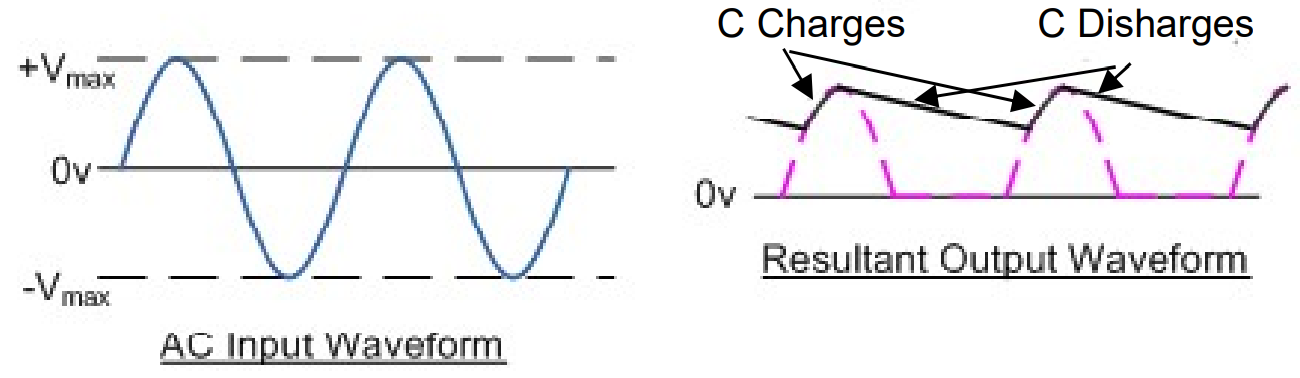
\includegraphics[width=1\columnwidth]{images/f2.png}
    \caption{Half-wave rectifier with a capacitor filter --- input and output waveforms}
\end{figure}

When the rectifier output voltage is increasing, the capacitor gets charged to its peak voltage $V_m$. Just past that, the rectifier output voltage starts to fall. As the source voltage decreases below $V_m$ , the capacitor will try to send the current back to diode making it reverse biased. Thus the diode separates/disconnects the source from the load and hence the capacitor will discharge through the load until the source voltage becomes more than the capacitor voltage. The diode again starts conducting and the capacitor is again charged to the peak value $V_m$ and the process continues. 

The decay is seen is the exponential decay of any capacitor is charging through a load resistor. The extent to which the capacitor voltage drops depends on the capacitance and the amount of current drawn by the load --- these two factors effectively form the RC time constant for voltage decay. A proper combination of large capacitance and small load resistance can give out a steady output.